\documentclass{article}
\usepackage[pdfcreator={LaTeX}]{hyperref}
\usepackage{graphicx}
\usepackage[utf8]{inputenc} 
\usepackage[ngerman]{babel}


\usepackage{tikz}
\usetikzlibrary{arrows,shadows}
\usepackage{pgf-umlsd}


\begin{document}
\begin{titlepage}

\begin{center}
\textbf{\textsc{\LARGE Implementierungsbericht}}

{\large \today}

\vspace{2cm}
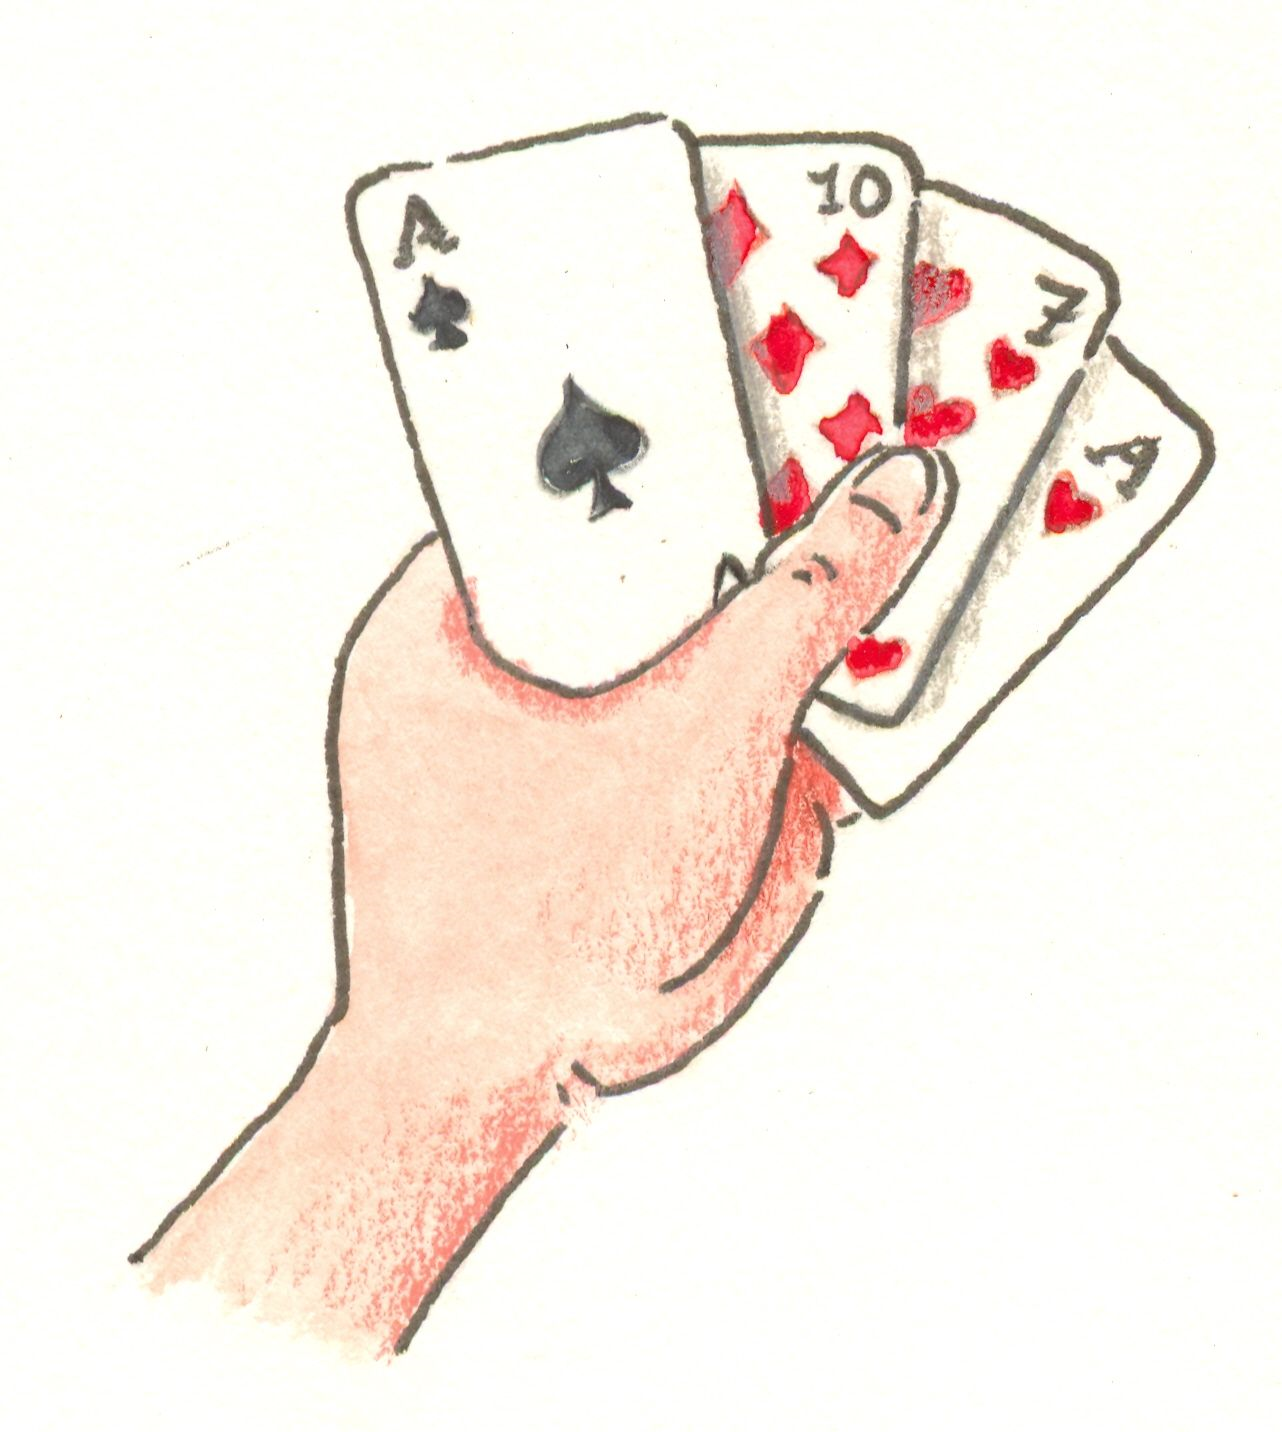
\includegraphics{kartenspiel}
\ \\
\ \\

\textbf{\textsc{\LARGE NET-WizHearts}}
\vspace{2cm}

\begin{tabular}{|c|c|c|}\hline
   Phase & Verantwortlicher & E-Mail \\ \hline\hline
   Pflichtenheft & Alina Meixl &  alina@meixl.de \\ \hline
   Entwurf & Viktoria Witka & witkaviktoria@freenet.de \\ \hline
   Spezifikation & Daniel Riedl & dariedl14@yahoo.de \\ \hline
   Implementation & Andreas Altenbuchner& a.andi007@gmail.com\\ \hline
   Verifikation & Patrick Kubin & kubin@fim.uni-passau.de\\ \hline
   Präsentation & w& w\\ \hline
 \end{tabular}

\end{center}

\end{titlepage}

\tableofcontents
\newpage

\section{Einleitung}
Dieses Dokument ist eine Dokumentation der Implementierungsphase. In Folgenden werden Änderungen aufgezählt, die seit der letzten Phase entstanden sind, des Weiteren wird eine Übersicht gegeben über die zuvor festgelegten Milestones und die tatsächliche Umsetzung dieser Aufteilung.

\section{Änderungen gegenüber der Spezifikation}

\subsection{Client}

\begin{itemize}
\item  \textbf{LanguageInterpreter:}  \textit{Neu hinzugefügte Klasse}: Wird verwendet, um Fehlermeldungen, die vom Server gesendet werden zu interpretieren und in der korrekten Sprache auszugeben.
\end{itemize}

\subsection{View}

\begin{itemize}
\item \textbf{Login:} \textit{hinzugefügt}: getUsername(), getServerAdress()
\item \textbf{Lobby:} \textit{hinzugefügt}: getChosenGameName(), getChatMessage(), hasPWChosenGame()
\item \textbf{CreateWindow:} \textit{entfernt}: addLeaveButtonListener(), addRulesetSelectionListener(); \textit{hizugefügt}: setRulesetTypes(), getGameName(), hasPassword(), getPassword(), getSelectedRulesetType()
\item \textbf{GameLobby:} \textit{hinzugefügt}: getChatMessage(), getSelectedPlayer()
\item \textbf{Game:} \textit{hinzugefügt}: getChatMessage(), addChatMessageListener() \textit{geändert}: makeTrickGameBoard()
\end{itemize}

\subsection{Ruleset}

\begin{itemize}
\item \textit{hinzugefügt} \textbf{DiscardedCard:} ;

\item \textit{hinzugefügt} \textbf{EmptyCard:};

\item \textbf{WizardCard:} \textit{hinzugefügt}: changeSorcererColour ();

\item \textbf{GameState:} \textit{hinzugefügt}: madeTrick(), restartDeck (), newRound(); \textit{gelöscht}: getNumberOfPlayedCards(), getCardsLeftInDeck()

\item \textbf{ServerRuleset} \textit{hinzugefügt}: updatePlayers (), getPlayedCards (), startRound(); 

\item \textbf{ServerWizard} \textit{hinzugefügt}: trumpColour; 

\item \textbf{ServerHearts:} \textit{hinzugefügt}: swapLeft(),swapRight(),swapAcross(), swap
\textit{geändert}: getWinners(),  ;
\end{itemize}

\subsection{Server}

\begin{itemize}
\item  \textbf{LoginServer:}  \textit{Neu hinzugefügte Klasse, erbt von Server}: Sie ist für das Zustabdekommen von Clientverbindungen zuständig. \textit{Attribute}:  Thread clientListenerThread,  LobbyServer lobby; \textit{Methoden}: receiveMessage(Player player, ComLoginRequest login), disconnectPlayer()
\item  \textbf{GameServer:} \textit{hinzugefügt}: quitGame(), getGameMasterName(), getPassword(), sendRulesetMessage(String player, RulesetMessage message), broadcastRulesetMessage(RulesetMessage message), sendWarning(String player, WarningMsg warning), broadcastWarning(WarningMsg warning) \textit{entfernt}: receiveMessage(Player player, ComClientQuit quit)
\item  \textbf{GameServerRepresentation:} \textit{implementiert jetzt Serializable}
\item  \textbf{LobbyServer:} \textit{entfernt}: innere Klasse ClientListenerThread, Set<Player> noNames, ServerSocket socket, receiveMessage(Player player, ComClientQuit quit ), receiveMessage(Player player, ComLoginRequest login); \textit{hinzugefügt}: addPlayerToGame(Player player, GameServer game), getNames()
\item  \textbf{ClientListenerThread:} erbt jetzt von Thread  \textit{hinzugefügt}: boolean waiting, ServerScocket socket, LoginServer server
\item  \textbf{Player:}  erbt jetzt von Thread  \textit{hinzugefügt}: Socket connection, boolean run, closeConnection(); \textit{geändert}: getName() heißt getPlayerName(), setName() heißt setPlayerName()
\item  \textbf{Server:} \textit{hinzugefügt}: eine receiveMessage Methode für jedes ComObject, das vom Server empfangen werden soll; \textit{geändert}: handleIOException heißt jetzt disconnectPlayer()
\item  \textbf{ServerMain:} \textit{hinzugefügt}: Attribut LoginServer loginServer
\end{itemize}

\subsection{ComObjects}

\begin{itemize}
\item 
\end{itemize}

\newpage

\section{Vergleich: Implementierungsplan und Realität}

\subsection{Änderungen am Plan}
\begin{itemize}
\item Zuständigkeit von Arbeitspaket Client(Lobby) wurde von Patrick an Andi gegeben, um die Arbeitszeiten anzugleichen
\item Zuständigkeit von Arbeitspaket Ruleset(Wizard-Client) wurde von Patrick/Andi and Daniel gegeben, um die Arbeitszzeiten anzugleichen
\end{itemize}

\subsection{Milestone 1}

\begin{tabular}{|c|c|c|c|c|}\hline
   Bereich & angen. Dauer & tats. Dauer & Abweichung & Begründung \\ \hline\hline
   View(Login+Lobby) & 8 Stunden & 4 Stunden & 50\% & (1) \\ \hline
   View(Create+Join) & 8 Stunden & 5 Stunden & 37,5\% &\\ \hline
   View(GameLobby) & 8 Stunden & 3 Stunden & 62,6\% &\\ \hline
   Model(Login) & 8 Stunden & 8,5 Stunden & (-) 6,25\% & (2) \\ \hline
   Client(Lobby) & 8 Stunden &  6,5 Stunden & 18,75\% &\\ \hline
   Client(Create+Join) &  8 Stunden & 6 Stunden & 25\% &\\ \hline
   Client (GameLobby) &  8 Stunden & 10 Stunden & (-) 25\% &\\ \hline
   Client (Game) & 14  Stunden &  12 Stunden & 14,3\% &\\ \hline
   Client (Wizard) & 6 Stunden & 0 Stunden & 100\% &\\ \hline
   Client (Hearts) & 4 Stunden & 0 Stunden & 100\% &\\ \hline
   Server(Login) & 16 Stunden & 6 Stunden & 62,5\% & (3) \\ \hline
   Server(Lobby) & 8 Stunden & 3 Stunden & 62,5\% &\\ \hline 
   Server(Create+Join) & 12 Stunden & 6 Stunden & 50\% &\\ \hline 
   Ruleset(Daten) & 20 Stunden & 5 Stunden & 25\% & (4) \\ \hline 
   Ruleset(ServerWizard) & 30 Stunden & 20 Stunden & 33,4\% &\\ \hline 
   Ruleset(ServerHearts) & 30 Stunden & 15 Stunden & 50\% &\\ \hline 
 \end{tabular}

\begin{itemize}
\item \textbf{(1)} Es waren noch Code-Teile aus der Pflichtenheft-Phase vorhanden. \\
\item \textbf{(2)} Login mehrmals umgebaut um die Tests aus dem Pflichtenheft zu erfüllen. \\
\item \textbf{(3)} Viele der ComObjects waren bereits fertig. \\
\item \textbf{(4)} Wurde hauptsächlich schon in Spezifikationsphase implementiert. \\
\end{itemize}

\subsection{Milestone 2}

\begin{tabular}{|c|c|c|c|c|}\hline
   Bereich & angen. Dauer & tats. Dauer & Abweichung & Begründung\\ \hline\hline
   View(Game) & 20 Stunden & 18,5 Stunden & 7,5\% &\\ \hline 
   Server(GameLobby) & 10 Stunden & 5 Stunden & 50\% &\\ \hline
   Ruleset(ClientWizard) & 6 Stunden & 5 Stunden & 16,7\% &\\ \hline 
   Ruleset(ClientHearts) & 6 Stunden & 5 Stunden & 16,7\% &\\ \hline 
   Handbuch & - & 5 Stunden & - &\\ \hline 
 \end{tabular}

\subsection{Milestone 3}

\begin{tabular}{|c|c|c|c|c|}\hline
   Bereich & angen. Dauer & tats. Dauer & Abweichung & Begründung\\ \hline\hline
   View(WizardWindows) & 4 Stunden & 2,5 Stunden & 37,5\% &\\ \hline
   View(HeartsWindows) & 4 Stunden & 2 Stunden & 50\% &\\ \hline
   Server(Game) & 4 Stunden & 2,5 Stunden & 37,5\% &\\ \hline
   Client(LanguageInterpreter) & - & 2 Stunden & - &\\ \hline
   Karten & - & 4 Stunden & - &\\ \hline
   Handbuch & - & 2 Stunden & - &\\ \hline
 \end{tabular}
 
\subsection{Finale Phase}
\begin{tabular}{|c|c|c|c|c|}\hline
   Bereich & angen. Dauer & tats. Dauer & Abweichung & Begründung\\ \hline\hline
 
 \end{tabular}

\end{document}
